\documentclass{sig-alternate}
\usepackage{epsfig}

\title{Cache Aware Optimization of Stream Programs}
\numberofauthors{1}
\author{
	Janis Sermulins, William Thies, Rodric Rabbah, and Saman Amarasinghe\\
	\small MIT Computer Science and Artificial Intelligence Laboratory\\
	\small \{janiss, thies, rabbah, saman\}@csail.mit.edu
}
\begin{document}

\maketitle

\begin{abstract}
Applications that are structured around some notion of a "stream"
are becoming increasingly important and widespread.  There is
evidence that streaming media applications are already consuming
most of the cycles on consumer machines \cite{Rix98}, and their
use is continuing to grow.  {\StreamIt} is a language and compiler
specifically designed for modern stream programming.  Despite the
prevalence of these applications, there is surprisingly little
language and compiler for practical, large-scale stream
programming.  {\StreamIt} is a language and compiler specifically
designed for modern stream programming.  The {\StreamIt} langauge
holds two goals: first, to provide high-level stream abstractions
that improve programmer productivity and program robustness within
the streaming domain; second, to serve as a common machine
language for grid-based processors.  At the same time, {\StreamIt}
compiler aims to perform stream-specific optimizations to achieve
the performance of an expert programmer.  This thesis develops
several techniques for scheduling execution of {\filters} in
{\StreamIt}.  The work focuses on correctness as well as
minimizing buffering requirements and stored schedule size.

\end{abstract}

\section{Introduction}

The domain of stream programs is important because it stands at the
intersection of trends in applications and architectures.  Stream
programming naturally represents applications such as audio, video,
digital signal processing, and data analysis; applications that are
increasing prevalent as computing moves towards data-centric
applications and to the mobile and embedded space.  Also, by virtue of
their structure -- a graph of independent computational nodes (termed
{\it filters}) with explicit and regular communication -- stream
programs are a natural fit for exploiting coarse-grained parallelism
suitable for multicore architectures.  The interest in streaming
applications has spawned a number of streaming languages that target
the streaming domain, including StreamIt~\cite{streamitcc},
Brook~\cite{brook04}, Cg~\cite{cg03},
SPUR~\cite{spur05samos}, Spidle~\cite{spidle03}, Lime~\cite{lime10},
and SPL~\cite{spl09}.

In a stream program, filters define an atomic execution step that
repeats for many iterations; each execution step discards a number of
data items from filter's input edge.  Often, a filter does not discard
all the data items that it read for the current execution step,
requiring these inspected (but not discarded) items for a future
iteration (or iterations) of the filter.  This type of filter is
described as performing a sliding window computation on its
input. Sliding window computations are prevalent in stream programs.
Examples of sliding window computations include FIR filters; moving
averages and differences; error correcting codes; motion estimation;
and network packet inspection.  A recent study of a large streaming
benchmark suite written in the StreamIt programming language finds
that 17 of the 30 real-world benchmarks include at least one filter
that performs a sliding window computation~\cite{streamit-suite}.


Figure~\ref{fig:fir-nopeeking} shows how to perform a sliding
window FIR filter via state carried between iterations of a filter.
This implementation is difficult for the compiler to analyze and
reason about.  Some programming languages (e.g., Brook, Lime,
StreamIt, and IBM SPL) go so far as to include idioms that directly
represent sliding window computation, allowing the programmer to
specify, for each filter, the size of the window and the number of
items discarded after an execution of the filter.
Figure~\ref{fig:fir-peeking} shows how language extensions of the
StreamIt programming language elegantly expose sliding windows for
compiler analysis and optimization.

A goal of stream programming is to directly expose to the software
layer the necessary information to enable automatic management of
coarse-grained parallelism.  Stream programs expose multiple forms of
parallelism: pipeline parallelism that exists between producers and
consumers; task parallelism that exists between pairs of filters on
parallel branches of the stream graph; and data parallelism that
exists when a filter is stateless and can thus be replicated.  Data
parallelism is the most attractive, as it provides load-balanced and
limitless parallelism (as long as input data is available).  A filter
that is stateful, and cannot be data-parallelized, becomes a limit to
parallelization scalability, as the work of that filter cannot be
divided; the most load-intensive stateful filter becomes a
bottleneck.

This paper presents a compiler framework for data-parallelizing
filters that perform sliding window computations when the properties
of the sliding window can be calculated statically.  If sliding window
filters required state, this state would represent a new
parallelization bottleneck.  Sliding windows are the bottleneck in 11
of the 17 real-world benchmarks in the StreamIt Benchmark Suite that
contain sliding windows~\cite{streamit-suite}.  For example, examining
the Channelvocoder benchmark, this state would limit scalability to 18
cores, whereas our techniques scale to at least 64 cores.

Data-parallelizing a filter is performed via a transformation termed
{\it fission} (verb form {\it fiss})~\cite{streamit-asplos}.  Fission
is the process of data-parallelizing a stateless filter by duplicating
the filter a certain number of ways, assigning duplicates to distinct
cores, and correctly distributed input data to and collecting output
data from the duplicates.  The duplicated filters are referred to as
{\it products}.  When a sliding window is present, fission is
accomplished by duplicating certain input items since they are
required by multiple products.  This duplication translates into
inter-core communication, a limiting factor for scalability when
targeting multicore architectures.

Previous approaches duplicate each input data item to all products,
with products ignoring (decimating) items that are not
needed~\cite{streamit-asplos}.  We will show that this strategy limits
scalability for multicores by requiring too much inter-core
communication.  In contrast, our strategy precisely routes each input
item to the minimal set of product filters that requires the item.
Unlike previous work, our techniques are defined on
multiple input and multiple output filters, removing the need to
introduce synchronization filters that serialize data before and
after the product filters.  

Our techniques operate on {\it static-rate} stream graphs, meaning
that the number of items produced, the number of items consumed, and
the number of items inspected by each filter can be determined
statically.  Because of this property, a steady-state schedule of
filter firings can be calculated that does not grow buffers and can be
executed indefinitely~\cite{lee87}.  Our techniques are conscious of
the spatial locality between producers and consumers.  Our framework
includes techniques that can determine when spatial locality can be
increased by altering the steady-state schedule.  When applicable, our
techniques can reduce the overall sharing (and thus inter-core
communication) requirement to below a threshold percent of the total
input communication for each sliding window filter that is
data-parallelized. 

\begin{figure}[t]
\centering
\subfigure[]{\includegraphics[width=3.3in]{figures/fir-nopeeking.pdf}\label{fig:fir-nopeeking}}
\subfigure[]{\includegraphics[width=3.3in]{figures/fir-peeking.pdf}\label{fig:fir-peeking}}
\caption[Two implementations of an FIR filter.]{\label{fig:fir-code}
  Two StreamIt implementations of an FIR filter:
   (a) the non-peeking version implemented via a
  stateful circular buffer; and (b) the peeking version. Only steady-state implementation is
  given.}
\end{figure}

The framework presented is defined on a model of computation that is
agnostic of source language.  To evaluate our techniques we have
implemented them in the context of the StreamIt compiler
infrastructure~\cite{gordon-asplos06}.  Our transformations are guided
by the parallelization management techniques presented
in~\cite{gordon-asplos06}.  We employ 3 real-world benchmarks from the
StreamIt Benchmark Suite~\cite{streamit-suite} that include sliding
window computation.  We demonstrate the effectiveness of our
techniques by comparing them to previously published techniques on 2
multicore architectures: a 16-core SMP shared-memory multicore and the
64-core distributed-memory Tilera TILE64.  We show that
our techniques are required to achieve scalable parallelization on
both architectures, achieving a 6.7x mean speedup on the 16-core SMP
and a 1.8x mean speedup on the 64-core distributed memory multicore
over a previously published technique.

\subsection{Contributions}
This paper makes the following contributions:
\begin{itemize}
  % \myitem{Motivation for Exposing Sliding Windows in Stream
  %   Languages}: Without exposing sliding windows in the language, it
  % requires heroic effort by the compiler to analyze the access patterns
  % of such a filter. Without success, the compiler will not be able to
  % data-parallelize these filters.  This will prevent robust 
  % parallelization scalability for streaming applications.

  \myitem{Generalized Fission of Sliding Window Filters}: We present a
  transformation that fisses sliding window filters with multiple
  input and multiple outputs.  The technique also supports filters
  that with multiple schedules of execution.  General fission defines
  a precise pattern of communication of input data to the products
  that can be reasoned upon by our other techniques.

  \myitem{Sharing Reduction}: We are the first to present a technique
  that decides when it is possible to decrease the amount of sharing
  between fission products by altering the steady-state of a stream
  graph, thus decreasing inter-core communication.  The technique
  reasons about all the sliding window filters of the stream graph,
  and when possible, reduces the sharing requirement to below a given
  threshold percent of the total input of the filters. 

  \myitem{Data Parallelization of Stream Graph}: We present a
  framework for data-parallelizing all of the filters of a stream
  graph employing the fission transformation on individual filters and
  applying sharing reduction when possible.  This framework optimizes
  for spatial locality and enables the compiler to automatically and
  effectively manage parallelization across varying multicore
  architectures.

  \myitem{Enable Robust Parallelization Scaling for Multicores}: For
  streaming applications with sliding window computation, previously
  published data-parallelization transformations do not scale for our
  target multicores. Our techniques enable robust parallelization
  scalability by reducing inter-core communication.  We achieve a 17x
  mean parallelization speedup for a 16-core SMP and a 62.3x mean
  parallelization speedup for the 64-core TILE64 across our benchmarks.

\end{itemize}

% \begin{figure}[t]
% \centering
% \begin{subfloat}
% \begin{minipage}[b]{0.45\textwidth}
% \eightpoint
% \begin{verbatim}
% float->float filter FIR(int N) {
%   int srcBuffer[N];
%   int srcEnd = 0; 
%   ...
%   work push 1 pop 1 {
%     srcBuffer[srcEnd] = pop();
%     float sum = 0;
%     for (int i=0; i<N; i++) {
%       sum += weights[i] * srcBuffer[(srcEnd + i + 1) % N];
%     }
%     push(sum);
%     srcEnd = (srcEnd + 1) % N;
%   }
% }
% \end{verbatim}
% \vspace{-8pt}
% \end{minipage}%
% \caption{ \label{fig:fir-nopeeking}}
% \end{subfloat}%
% \qquad
% \begin{subfloat}
% \begin{minipage}[b]{0.45\textwidth}
% \eightpoint
% \begin{verbatim}
% float->float filter FIR(int N) {
%   ...
%   work push 1 pop 1 peek N {
%     float sum = 0;
%     for (int i=0; i<N; i++) {
%       sum += weights[i] * peek(i);
%     }
%     push(sum);
%     pop();
%   }
% }
% \end{verbatim}
% \vspace{-18pt}
% \end{minipage}
% \caption{ \label{fig:fir-streamit}}
% \end{subfloat}
% \caption[Two implementations of an FIR filter.]{\label{fig:fir-code}
%   Two StreamIt implementations of an FIR filter:
%    \subref{fig:fir-nopeeking} the non-peeking version implemented via a
%   stateful circular buffer; and \subref{fig:fir-streamit} the peeking version. Only steady-state implementation is
%   given.}
% \end{figure}

\Section{StreamIt Programming Language}
\label{sec:streamit}

StreamIt~\cite{streamit-cc} is an architecture independent language
that is designed for stream programming. In StreamIt, programs are
represented as graphs where nodes represent computation and edges
represent FIFO-ordered communication of data over tapes. The language
features several novelties that are essential for large scale program
development. The language is modular, parameterizable, malleable and
architecture independent. In addition, the language exposes the
inherent parallelism and communication patterns that are prevalent in
streaming programs.

\begin{figure*}[t]
  \begin{minipage}[t]{4.0in}
    {
	\begin{scriptsize}
	  \begin{verbatim}
	    int->int filter ZigZagScan(int N, int[N] Order)
	    {
	        work pop N push N {
	        for (int i = 0; i < N; i++) {
	          int pixel = peek(Order[i]);
	          push(pixel);
	        }
	        for (int i = 0; i < N; i++) {
	          pop();
	        }
	      }
	    }
	  \end{verbatim}
	\end{scriptsize}
    }
    % \vspace{-3pt}
    \caption{Example filter implementing zig-zag scanning.}
    % \label{fig:zigzag-filter}
  \end{minipage}
  ~~\vrule~~
  \begin{minipage}[t]{3.0in}
    {  
	\begin{scriptsize}
	  \begin{verbatim}
	    int[64] Ordering = 
	      {00, 01, 05, 06, 14, 15, 27, 28,
	       02, 04, 07, 13, 16, 26, 29, 42,
	       03, 08, 12, 17, 25, 30, 41, 43,
	       09, 11, 18, 24, 31, 40, 44, 53,
	       10, 19, 23, 32, 39, 45, 52, 54,
	       20, 22, 33, 38, 46, 51, 55, 60,
	       21, 34, 37, 47, 50, 56, 59, 61,
	       35, 36, 48, 49, 57, 58, 62, 63};



	  \end{verbatim}
	\end{scriptsize}
    }
    % \vspace{-3pt}
    \caption{Example zig-zag order for filter.}
    \label{fig:zigzag-order}
  \end{minipage}
\end{figure*}

\SubSection{Filters as Programmable Units}
In StreamIt, the basic programmable unit is a {\it filter}. Each
filter contains a work function that executes atomically, popping
(i.e., reading) a fixed number of items from the filter input tape
and pushing (i.e., writing) a fixed number of items to the filter
output tape. A filter may also {\tt peek} at a given index on its
input tape without consuming the item; this makes it simple to
represent computation over a sliding window or performing permutations
on the input stream. The {\tt push}, {\tt pop}, and {\tt peek} rates
are declared as part of the work function, thereby enabling the
compiler to apply various optimizations and construct efficient
execution schedules. 

A filter is akin to a class in object oriented programming with the
work function serving as the main method. A filter is parameterizable,
and this allows for greater malleability and code reuse. An example
filter is shown in Figure~\ref{fig:zigzag-filter}. This filter
consumes a stream whose elements are of type {\tt int} and produces a
stream of the same type. It implements the zig-zag scanning pattern
used in the run-length encoding of quantized DCT coefficients (see
Figure~\ref{fig:zigzag}). Typically, the zig-zag scan operates on a
8x8 matrix. An instantiation of a filter can specify the matrix
dimensions, as well as the desired ordering. In MPEG, there are two
possible scan orders. The {\tt Order} parameter can define the
specific scan pattern that is desired. For example, to implement the
order shown in Figure~\ref{fig:zigzag}(a), the array is defined as
shown in Figure~\ref{fig:zigzag-order}.

In this example, the DCT matrix is represented as a unidimensional
stream. The filter peeks or inspects the elements and copies them to
the output stream in the specified order. Once all the DCT
coefficients are copies, the input stream is deallocated from the tape
with a series of pops.

\begin{figure}[t]
\begin{center}
%\vspace{-24pt}
% \framebox{
 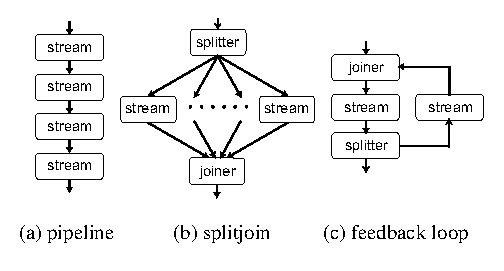
\includegraphics[scale=1, angle=0]{./constructs-eg.eps}
%}
% \vspace{-6pt}
% \nocaptionrule
 \caption{Hierarchical streams in StreamIt.}
 \label{fig:containers}
\end{center}
\end{figure}

\SubSection{Hierarchical Streams}
In StreamIt, the application developer focuses on the hierarchical
assembly of the stream graph and its communication topology, rather
than on the  explicit management of the data buffers between filters.
StreamIt provides three hierarchical structures for composing filters
into larger stream graphs (see Figure~\ref{fig:containers}).

\paragraph{Pipeline.}
The {\it pipeline} stream construct composes streams in sequence, with
the output of one connected to the input of the next.  An example of a
pipeline appears in Figure~\ref{fig:decoder-pipeline}. A pipeline is a
single input to single output stream. The decoding pipeline in the
figure consists of three streams. The first is a filter which zig-zag
unorders the input stream, and prepares the data for the inverse
quantization and DCT. The output of the filter is consumed by a stream
named {\tt IQ} which is a pipeline itself (not shown). This example
illustrates the hierarchical nature of stream composition in
StreamIt. The {\tt IQ} pipeline performs the inverse quantization, and
produces an output stream that is in turn consumed by another stream
which performs the inverse DCT. As in the case of a filter, pipelines
are also parameterizable.

\begin{figure*}[t]
  \begin{scriptsize}
    \begin{verbatim}
	int->int pipeline Decode()
	{ 
	  int Order[64] = {...};     // initialized as shown earlier
	  add ZigZagScan(64, Order);
	  add IQ();                  // inverse quantization
	  add IDCT(8, 8);            // inverse DCT (8x8 matrix)
	}
    \end{verbatim}
  \end{scriptsize}
  % \vspace{-3pt}
  \caption{Example MPEG decoder pipeline.}
  \label{fig:decoder-pipeline}
\end{figure*}

The {\tt add} keyword in StreamIt constructs the specified stream
using the input parameters. The {\tt add} statement may only appear in
non-filter streams.  In essence, filters are the leaves in the
hierarchical construction, and composite nodes in the stream graph
define the encapsulating containers. This allows for modular design
and development of large applications, thereby  promoting
collaboration, increasing code reuse, and simplifying debugging.

\paragraph{Split-Join.}
The {\it splitjoin} stream construct distributes data to a set of
parallel streams, which are then joined together in a roundrobin
fashion. In a splitjoin, the {\it splitter} performs the data
scattering, and the {\it joiner} performs the gathering. A splitter is
a specialized filter with a single input and multiple output
channels. On  every execution step, it can distribute its output to
any one of its children in either a {\it duplicate} or a {\it
roundrobin} manner. For the former, incoming data are replicated to
every sibling connected to the splitter. For the latter, data are
scattered in a roundrobin manner, with each item sent to exactly one
child stream, in order. The splitter type and the weights for
distributing data to child streams are declared as part of the syntax
(e.g., \texttt{split duplicate} or \texttt{split
roundrobin($w_1,\ldots,w_n$)}). The splitter counterpart is the
joiner. It is a specialized filter with  multiple input channels but
only one output channel. The joiner gathers data from its predecessors
in a roundrobin manner (declared as part of the syntax) to produce a
single output stream.

\begin{figure*}[t]
  \begin{scriptsize}
    \begin{verbatim}
	// N = macroblock size + motion vector data size;
	// W = picture width (resolution in pixels);
	// H = picture width (resolution in pixels);

	int->int splitjoin YCrCbDecoding(int N, int W, int H)
	{
	  // 4:2:0 chroma format
	  split roundrobin(4*N, 1*N, 1*N);

	  add LuminanceChannel  (W, H);
	  add ChrominanceChannel(W, H);
	  add ChrominanceChannel(W, H);

	  join roundrobin(1, 1, 1);  
	}
    \end{verbatim}
  \end{scriptsize}
  % \vspace{-3pt}
  \caption{Example MPEG decoder splitjoin.}
  \label{fig:decoder-sj}
\end{figure*}

The splitjoin stream is a convenient and natural way to represent
parallel computation. For example, when the decoder performs the
luminance and chrominance channel processing, the computation can
occur in parallel. In StreamIt, this is expressed as shown in
Figure~\ref{fig:decoder-sj}. The input stream contains the
macroblock data along with the parsed motion vectors. The data is
partitioned and passed to one of three decoding channels, with $4N$
items assigned to the first stream, $N$ items to the second, and $N$
items to the third. The three streams reconstruct the original
pictures with respect to the different color channels, and their
output is combined by the joiner to produce the final decoded picture.

\paragraph{Feedback Loop.}
StreamIt also provides a {\it feedback loop} construct for introducing
cycles in the graph. This stream construct is not used in the decoder,
but may be used in the MPEG encoder.

\paragraph{XXX: need to introduce messaging and talk about it.}
\section{Cache Model for Streaming}
\label{sec:cache-model}

In this section we describe a simple and intuitive cache model to
estimate the instruction and data cache behavior given an execution
ordering of the filters in the stream graph.

The model is based on the notion of a filter reuse distance which is 
based on LRU stack distance~\cite{mattson70}. We develop the model
first for the instruction cache, and then subsequently generalize it to
account for the data cache.

\subsection{Instruction Cache}

A {\it filter execution trace} is a sequence of 
filter work functions executions: $T = f_0 f_1 ... f_n$; $f_i$ represents the
execution of filter $f$ at logical time $i$.
The filter {\it instruction reuse distance} ($\mt{IRD}$) is defined as the
number of unique instructions that are referenced between two
instances of the same work function. Formally, we define $phase(f_i)$
as the sequence $f_i ... f_l$ ($i < l$) of work functions occurring in
$T$ such that $f_i = f_l$ and nowhere else (i.e., $f_i \neq f_k$
$\forall{k}~~s.t.~~i < k < l$). The $\mt{IRD}(f_i) = \sum I(f_j)$ over all
distinct filters occurring in $phase(f_i)$, and $I(f)$ equals the code
size of a filter $f$. Based on this reuse metric, we define an
instruction-cache-miss step function $\mt{IMS}(f_i)$ such that:
\begin{equation}
\label{eq:ims}
  \mt{IMS}(f_i) =
    \begin{cases}
      0& \text{if $\mt{IRD}(f_i) \leq C_I$; hit/no cache refill},\\
      1& \text{else; a miss/(some) cache refill}.\\
    \end{cases}
\end{equation}
Note that if $f_i$ is the last occurrence of a filter $f$ in the trace,
then $IMS(f_i) = 0$. In Equation~\ref{eq:ims}, $C_I$ represents a
constant proportional to the instruction cache size.

We do not account for the cold start
effects of an execution trace. This does not affect our model, and can
be easily remedied if necessary. To see why this is so, consider the
following two execution traces which represent the executions of work
functions for two filters \texttt{A} and \texttt{B}:
$T_1 = \texttt{A}_1\texttt{A}_2\texttt{B}_3\texttt{B}_4$
and 
$T_2 = \texttt{A}_1\texttt{B}_2\texttt{A}_3\texttt{B}_4$.
In both 
traces, the number of cold starts is the same (i.e., two in all).

What our reuse metric quantifies is the number of misses when a specific work
function is reinvoked. For example, assume that each filter is of the exact
size: $I(\texttt{A}) = I(\texttt{B}) = \lceil{C_I / 2}\rceil + 1$;
that is, the combined instruction working sets of both filters exceeds
the instruction cache, although each filter has a code size that is
smaller than the cache size. Naturally, we expect the trace $T_1$ to
suffer one cold start miss and no other misses for filter \texttt{A}
(and similarly for the other filter). Our model is in accord with
intuition:  $\mt{IMS}(\texttt{A}_1) = 0$ since
the $\mt{IRD}(\texttt{A}_1) < C_I$.

In the case of trace $T_2$, we know that since the combined
instruction working sets of the filters exceeds the cache size, when
filter \texttt{B} is invoked following \texttt{A}, it evicts part of
filter \texttt{A}'s instruction working sets. Hence when we transition
back to run filter \texttt{A}, we have to refetch certain
instructions, but in the process, we replace parts of filter
\texttt{B}'s working sets. Hence, we have suffered one cold start miss,
and one capacity miss for filter \texttt{A}, and similarly for
\texttt{B}. Our model is again in accord with intuition: 
$\mt{IMS}(\texttt{A}_1) = 1$ since
the $\mt{IRD}(\texttt{A}_1) > C_I$. Note that the
amount of refill is proportional to the number of cache lines that are
replaced when swapping filters, and as such, we may wish to adjust
our cache miss step function. One simple variation is to allow for
some partial replacement without unduly penalizing the overall value
of the metric. Namely, we can allow the constant $C_I$ to be some
fraction greater than the actual cache size. Alternatively, we can use
a more complicated miss function with a more uniform probability
distribution.

Using the metrics above, we can estimate the instruction-cache miss
rate $(IMR)$ as $\sum IMS(f_i)$ over all $f_i$ in the trace, divided
by the size of the trace. Note that different execution orderings for
the same stream graph lead to traces of the same size and hence the
comparisons are fair. The model allows us to rank the quality of an
execution ordering, with scheduling decisions that boost temporal
locality yielding miss rates closer to zero (and schedules that do not
exploit temporal locality yielding traces with miss rates closer to
one).

Our model predicts that scaling is always beneficial from an
instruction-cache point of view. As a reminder, by scaling, we mean
that a filter's work function is run for a greater number of times in
the steady state before transitioning to the next filter in the
graph. Hence for example, a program that would generate a trace $T_2$
might be as follows:
{\small
\begin{verbatim}
run_steady_state() {
  for (i = 0; i < 1; i++) A_work();
  for (i = 0; i < 1; i++) B_work();
}
\end{verbatim}}
\noindent but a scaled program that increases temporal locality is as follows:
{\small
\begin{verbatim}
run_steady_state() {
  for (i = 0; i < M * 1; i++) A_work();
  for (i = 0; i < M * 1; i++) B_work();
}
\end{verbatim}}
\noindent where \texttt{M} (the multiplicity factor) is an integer greater than
one. From our model, it is easy to see that scaling reduces the number
of misses for a given filter $f$ from $K$ to $\frac{K}{\texttt{M}}- 1$, where $K =
\sum \mt{IMS}(f)$ for all occurrences of $f$ in  the execution trace.

\subsection{Data Cache}

As noted earlier, we can not arbitrarily scale the execution frequency
of a filter without also considering how scaling might impact
the data buffer sizes between filters. In this regard, a filter's
output buffer size is also constrained by the amount of state that a
filter retains with every execution of its work function.

Clearly if a filter has any static data (e.g., state information or
coefficient arrays), then it is prudent to maximize their temporal
access locality. We can define a data-cache miss rate ($\mt{DMR}$) based on
a derivation similar to that for the instruction-cache miss rate:
replace $C_I$ with $C_D$ in Equation~\ref{eq:ims}, and $I(f_i)$ with
$S(f_i)$ when calculating the {\it data reuse distance} ($\mt{DRD}$). 
Here, $C_D$ represents a constant proportional to the data cache size,
and $S(f)$ represents the total size of the static data in the
specified filter.

The presence of static data in a filter implies that we have to limit
the scaling of a filter $f$ such that it does not require more than $C_D -
S(f)$ bytes of buffer space for reading and writing data; otherwise
the data working sets of the filter will overflow the cache and we lose
producer-consumer locality. The buffer requirements are represented by
$Y(f_i)$, and the data-cache model accounts for the dynamic data
requirements by adjusting the data reuse distance as follows:
$\mt{DRD}(f_i) = \sum (S(f_i) + Y(f_i))$ over all distinct filters occurring
in $phase(f_i)$.

Intuitively, the dynamic data accounts for the size of the buffer
required for writing new values, as well as the size of the buffer
necessary for reading values. It also adjusts for any
producer-consumer locality since the output buffer of one filter is
also the input buffer of its neighbor in the stream graph. What this
measure tells us is that we can scale the execution of a filter as
long as its buffer requirements (for reading and writing) do not
exceed the cache, and furthermore, as long as the input-output rates
between producer consumer pairs are not grossly mismatched. Managing the buffer 
requirements is important and motivates a series of cache
optimizations discussed in the next section. In the case of rate
mismatch, the metric tells us that the effective cache size is
reduced, or in other words, the data that is left over after a
producer-consumer firing must be preserved until a future occurrence of
the same pair of filters. This translates to lower data locality and
degrades cache performance.

Mathematically, the dynamic data measure is defined as:
\begin{eqnarray}
  \nonumber
  Y(f_i) &=&\sum_{f_k} min(W(f_k), U(f_k) \times A(f_k)) + \\
  \nonumber
	   &&\sum_{f_k} min(R(f_k), O(f_k) \times A(f_k)) - \\
  \nonumber
         &&\sum_{f_s} min(R(f_s), O(f_s) \times A(f_s))
\end{eqnarray}
with $W(f)$ equal to the output buffer size reserved for writing data, $R(f)$
equal to the input buffer size reserved for reading data, $U(f)$ equal to the
{\tt push} rate (in bytes) of the filter, $O(f)$ equal to the {\tt pop} rate (in
bytes) of the filter, and $A(f)$ equal to the number of occurrences of
filter $f$ in $phase(f_i)$. Also note that the $Y(f_i)$ is defined
over all distinct occurrences of $f_k$ in the phase, and $f_s$
represents the filter that consumes the data produced by $f_k$ (i.e.,
it is $f_k$'s successor in the stream graph, and $f_k$--$f_s$
constitute a producer-consumer pair; $f_s$ is unique unless $f_k$ is a splitter).

The first summand in the equation above quantifies the address space
accessed for writing data. It is  equal to the lesser of the buffer size
reserved for output, and the total number of items produced by
the filter (i.e., the push rate multiplied by the number of times the
work function fired in the phase); this avoids over estimating the
address space when an exceedingly large buffer is reserved but only a
portion of it is used for writing in a phase.

The second term in the equation quantifies the referenced address space 
for reading the input data. This term is also the lesser of two
values: the input buffer size, and the total number of bytes referenced for
reading data.

The third term avoids double counting since the output buffer of one
filter is also the input buffer of its successor in the stream
graph. The term quantifies the amount of data that is consumed by the
producer's successor (which therefore releases a portion of the
address space for use by other filters in the phase).

\subsection{Remarks}

Note  that we can  combine the  instruction and  data cache  miss rate
equations to yield one measure that estimates the temporal locality of
a streaming computation.

Also note that while we use  an execution trace to describe our model,
it  is possible  to  calculate  the instruction  and  data cache  miss
metrics at  compile time.  To do so,  we can leverage  the hierarchical
StreamIt   representation  that  dictates   the  ordering   of  filter
executions.

\section{Cache Optimizations}
\label{sec:cache-opt}

In this section we two cache-aware optimizations that
are geared toward the cache behavior of streaming programs. First, we
describe {\it multiplicity scaling} which 
scales a steady state to improve instruction locality, subject to the
data working set constraints of the actors in the stream graph.
Second, we describe {\it cache-aware fusion} which performs a series
of granularity adjustments to the actors in the steady state. The
fusion serves to $(i)$ reduce
the overhead of switching between actors, $(ii)$ create coarser
grained actors for multiplicity scaling, and $(iii)$ enable novel
buffer management techniques between fused actors, as detailed
Section~\ref{sec:buffer}.

\subsection{Multiplicity Scaling}
We have already alluded to multiplicity scaling in previous
sections. As the instruction cache model shows, increasing the number
of consecutive firings of the same actor leads to lower miss
rates. However, scaling increases the data buffers that are maintained
between actors. Thus it is prudent that we account for the data
working set requirements as we scale a steady state.

\begin{figure}[t]
\begin{center}
\framebox{\parbox{3.25in}{
\mbox{} ~~~~// {\it Returns a multiplicity factor for steady state $S$} \\
\mbox{} ~~~~// - $C_D$ is the data cache size\\
\mbox{} ~~~~// - $\alpha$ is the fraction of $C_D$ dedicated for I/O $(0 < \alpha)$\\
\mbox{} ~~~~// - $p$ is the desired percentile of all actors to be\\
\mbox{} ~~~~// satisfied by the chosen multiplicity $(0 < p \le 1$)\\
\mbox{} ~~~~{\bf calculateMultiplicity}($S$, $C_D$, $\alpha$, $p$) \{\\
\mbox{} ~~~~~~~{\bf create} $\mt{array}$ of size $|S|$ and {\bf initialize} all entries to 0\\
\mbox{} ~~~~~~~{\bf for} $i$ = 1 to $|S|$ \{ \\
\mbox{} ~~~~~~~~~~$X = S[i]$\\
\mbox{} ~~~~~~~~~~// calculate effective cache size\\
\mbox{} ~~~~~~~~~~$C = \alpha \times (C_D - \mt{State}(X))$\\
%\mbox{} ~~~~~~~~~~// estimate I/O requirements\\
%\mbox{} ~~~~~~~~~~$d = \mt{IO}(X)$\\
\mbox{} ~~~~~~~~~~// account for the I/O requirements and
\mbox{} ~~~~~~~~~~// calculate largest possible scaling for $X$\\
\mbox{} ~~~~~~~~~~$M_X = \lfloor C / \mt{IO}(X) \rfloor$\\
\mbox{} ~~~~~~~~~~// array indexed from 0 \\
\mbox{} ~~~~~~~~~~$\mt{array}[i - 1] = M_X$\\
\mbox{} ~~~~~~~\} \\
\mbox{} ~~~~~~~{\bf sort} $\mt{array}$ into ascending numerical order\\
\mbox{} ~~~~~~~$i = \mt{{\bf round}}((1-p) \times (|S| - 1))$ \\
\mbox{} ~~~~~~~return $\mt{array}[i]$\\
\mbox{} ~~~~\}
}}
\end{center}
\nocaptionrule
\caption{Algorithm for calculating the multiplicity factor.}
\label{fig:scaling-algo}
\end{figure}

Our approach is to scale the entire steady state by a single
multiplicity factor, with the constraint that only a small percentage
of the actors overflow the data cache. Our two-staged algorithm is
outlined in Figure~\ref{fig:scaling-algo}.

{\it First}, The algorithm calculates the largest
possible multiplicity  
for every actor in the steady state. To do this, it
adjusts the effective cache size that is reserved for an actor's
dynamic working set (i.e., data accessed via {\tt pop} and {\tt
push}). This adjustment allows us to control the fraction of the cache
that is used for reading and writing data---and affords some
flexibility in targeting various cache organizations.  For example,
architectures with highly associative and multilevel caches may benefit
from scaling up the effective cache size (i.e., $\alpha > 1$), whereas
a direct mapped cache that is more prone to conflicts may benefit from
scaling down the cache (i.e., $alpha < 1$). In our implementation, we
found $\alpha=2/3$ to work well. However, we note that tuning the
effective cache size is not only dependent on the underlying cache
organization, but also dependent on the instruction  working
set size, and the  I/O properties of the actors in the steady
state; this is an interesting issue that warrants further
investigation.

{\it Second}, it chooses the largest
factor that allows a fraction ($p$) of the steady state actors to be
scaled safely (i.e., the cache is adequate for their I/O
requirements).  For example, the algorithm might calculate
$M_\texttt{A} = 10$,
$M_\texttt{B} = 20$, 
$M_\texttt{C} = 30$, and 
$M_\texttt{D} = 40$, for four actors in some steady state. Thus,
scaling actor \texttt{A} beyond 10 consecutive iterations will cause
its dynamic I/O requirements to exceed the data cache. Therefore, the
largest $M$ that allows 90\% of the actors to be
scaled without violating the cache constraints is 10.
Similarly, to allow for the safe scaling of 75\% of the actors, the
largest factor we can choose is 20.

In our implementation, we use the 90-10 heuristic. In other words, we
set $p=90\%$. We empirically determined this value via a series of
experiments using our benchmark suite. Specifically, we varied the
multiplicity factor across a wide range of values,
and measured the resulting performance. We found that
increasing the threshold beyond 90\% leads to marginal
performance gains. Due to the limited space we cannot include all of
the collected data. However, the interested reader can find
the results in a thesis by one of the authors~\cite{janis-thesis}.


\subsection{Actor Coarsening}
In StreamIt, the granularity of actors is determined by the
application developer, according to 
the most natural representation of an algorithm. When compiling to a
cache-based architecture, the presence of a  large number of actors
exacerbates the transition overhead between work functions.
It is the role of the compiler  to adjust the granularity of
the stream graph to mitigate the execution overhead.

In this section we describe an actor coarsening technique we refer to
as {\it cache aware fusion} (CAF). When two actors are fused, they
form a new actor whose work function is equivalent to its constituents.
For example, let an actor \texttt{A} fire $n$
times, and an actor \texttt{B} fire $2n$ times per steady state:
$S^n=(\texttt{A}^n\texttt{B}^n\texttt{B}^n)$. A fused actor \texttt{F}
is formed that is equivalent to one firing of \texttt{A} and two 
firings of \texttt{B}; \texttt{F} fires $n$ times per steady state
$(S^n=(\texttt{F}^n))$.  In other terms, the work
function for actor \texttt{F} inlines the work functions of
\texttt{A} and \texttt{B}.

When two actors are fused, their executions are scaled such that the output
rate of one actor matches the input rate of the next. In the example,
\texttt{A} and \texttt{B} represent a producer-consumer pair of
filters within a pipeline, with filter \texttt{A}  
pushing two items per firing, and \texttt{B} popping one item per
firing. The fusion implicitly scales the execution of \texttt{B} so
that it runs twice for every firing of \texttt{A}.

%Fusion is important because it leads to coarser grained actors with
%I/O rates that are more closely matched to their
%neighbors. Furthermore, the fused actors themselves become the target
%the execution scaling which results in better producer-consumer locality.

Fusion also reduces the overhead of switching between
work functions. In our infrastructure, the steady state is a loop that
invokes the work functions via method calls. Thus, every pair of fused
actors eliminates a method call (per invocation of the actors). The impact on
performance can be significant, but not only because method calls are
removed: the fusion of two actors also enables the compiler to
optimize across function boundaries. In particular, for actors that
exchange only a few data items, the compiler can allocate the data
streams to registers. 
%For example, in the example above, the values
%produced by \texttt{A} may be passed to \texttt{B} via registers, rather
%than through memory. 
The data channel between fused actors is
subject to special buffer management techniques as described in the
next section.

There are, however, downsides to fusion. First, as more and more
actors are fused, the instruction footprint can dramatically increase,
possibly leading to poor use of the instruction cache. Second, fusion
increases the data footprint when the fused actors maintain state
(e.g., coefficient arrays and lookup tables). Our fusion algorithm is
cache aware in that it is cognizant of the instruction and data sizes.

The CAF algorithm uses a greedy fusion heuristic to determine which filters
should be fused. It continuously fuses actors until the addition of
a new actor causes the fused actor to exceed {\it either} the instruction cache
capacity, or a fraction of the data cache capacity. For the latter, we
allow the state of the new fused actor to occupy up to 50\% of the
data cache capacity.

The algorithm leverages the hierarchical nature of the stream graph,
starting at the leaf nodes and working upward.  For pipeline streams,
the algorithm identifies the connection in the pipeline with the
highest steady-state I/O rate, i.e., the pair of filters that
communicate the largest number of items per steady state.  These two filters
are fused, if doing so respects the instruction and data cache constraints.
To prevent fragmentation of the pipeline, each fused filter is further
fused with its upstream and downstream neighbors so long as the
constraints are met.  The algorithm then repeats this process with the
next highest-bandwidth connection in the pipeline, continuing until no
more filters can be fused.  For splitjoin streams, the CAF algorithm
fuses all parallel branches together if the combination satisfies the
instruction and data constraints.  Partial fusion of a splitjoin is
not helpful, as the child streams do not communicate directly with
each other; however, complete fusion can enable further fusion in
parent pipelines.

%% This differs from that in
%% \cite{streamit-asplos} in that the algorithm
%% only considers vertical fusion (i.e., within a pipeline): horizontal
%% fusion is not beneficial from caching perspective. \framebox{Expand on this} \framebox{Emphasize order:  fuse then scale.}
%Second, since the 
%graph partitioning is limited to
%horizontal cuts, our actor coarsening optimizations employs a greedy
%algorithm instead of a dynamic programing methodology; this reduces
%compilation time. 

%% \begin{figure*}[t]
%% \begin{verbatim}
%% Pipeline:

%% Calculate number of partitions required for each child.
%% If for any child this is >1 then remember those partitions.

%% For each sequence (i..j) of children where for each child 
%% number of partitions is 1.

%% Interval(i,j) = "
%%     Find maximum bandwidth connection between children. (k, k+1)
%%     Consider partition (k..k+1) 
%%     If partition (k..k+1) does not satisfy the requirement then
%%         Call Interval(i,k) and Interval(k+1,j) to find two sets of partitions.

%%     Else Start with (k, k+1) fused try fusing up or down
%%         until can not fuse up and down let this be (l, m)
%%         Remember (l..m) as a partition.
%%         Use Interval(i,l) and Interval(m,j) to find partitions."

%% SplitJoin:

%% Consider splitter/joiner and all branches in a single partition.
%% If this satisfies requirements then return a single partion
%% else remember partitions corresponding to each branch as final
%% partitions.
%% \end{verbatim}
%% \caption{Pseudocode of a greedy algorithm to find partitions}
%% \label{fig:greedy}
%% \end{figure*}


\section{Buffer Management}
\label{sec:buffer}

\begin{figure}[t]
%% \begin{minipage}{1.7in}
%% \centering
%% \psfig{figure=fusion-pipeline.eps,width=0.7in}

%% \caption{Stream graph for a synthetic buffer test.\protect\label{fig:code-graph}}
%% \end{minipage}
%% \hspace{0.3in}
\centering
{\small
\begin{verbatim}
   void->void filter BufferTest {       
     int PEEK = 4;                      
     float[4] BUFFER;                   
     int push_index = 0;                
     int pop_index = 0;                 
                                        
     prework {                          
       for (int i=0; i<PEEK-1; i++) {   
         BUFFER[push_index++] = ... ;
       }                                
     }                                  
                                        
     work {                             
       // run Source                    
       BUFFER[push_index] = ... ;
       push_index = (push_index+1) & 3;              
                                        
       // run FIR                       
       float result = 0;                
       for (int i=1; i<PEEK; i++) {     
         result += i*BUFFER[(pop_index+i) & 3];    
       }                                
       pop_index = (pop_index+1) & 3;     
       print(result);                   
     }                                  
   }                                    
\end{verbatim}}
\vspace{-6pt}

\caption{Fused buffer test using modulation buffer management.\protect\label{fig:code-modulation}}
\end{figure}

\begin{figure*}
\begin{minipage}{2.2in}
\psfig{figure=arm-buf.eps,width=2.2in}
\caption{Performance of buffer management strategies on a StrongARM.\protect\label{fig:buf-arm}}
\end{minipage}
\hspace{0.1in}
\begin{minipage}{2.2in}
\psfig{figure=p3-buf.eps,width=2.2in}
\caption{Performance of buffer management strategies on a Pentium~3.\protect\label{fig:buf-p3}}
\end{minipage}
\hspace{0.1in}
\begin{minipage}{2.2in}
\psfig{figure=i2-buf.eps,width=2.2in}
\caption{Performance of buffer management strategies on an Itanium~2.\protect\label{fig:buf-itanium}}
\end{minipage}
\vspace{18pt}
\hrule
\begin{minipage}[t]{2.1in}
%% copy-shift
{\scriptsize
\begin{verbatim}


void->void filter BufferTest {
  int PEEK = 4;
  float[3] BUFFER;

  prework {
    for (int i=0; i<PEEK-1; i++) {
      BUFFER[i] = ... ;
    }
  }

  work {
    float[4] TEMP_BUFFER;
    int push_index = 3;
    int pop_index = 0;

    // copy from BUFFER to TEMP_BUFFER
    for (int i=0; i<3; i++) {
      TEMP_BUFFER[i] = BUFFER[i];
    }

    // run Source
    TEMP_BUFFER[push_index++] = ... ;
    
    // run FIR
    float result = 0;
    for (int i=1; i<PEEK; i++) {
      result += i*TEMP_BUFFER[pop_index+i];
    }
    pop_index++;
    print(result);

    // copy from TEMP_BUFFER to BUFFER
    for (int i=0; i<3; i++) {
      BUFFER[i] = TEMP_BUFFER[i+1];
    }
  }
}
\end{verbatim}}

\caption{Copy-shift strategy.\protect\label{fig:copy-shift}}
\end{minipage}
~~\vrule~~
\begin{minipage}[t]{2in}
%% copy-shift + scalar-replacement
{\scriptsize
\begin{verbatim}


void->void filter BufferTest {
  int PEEK = 4;
  float[3] BUFFER;

  prework {
    for (int i=0; i<PEEK-1; i++) {
      BUFFER[i] = ... ; 
    }
  }

  work {
    float TEMP_BUFFER_0;
    float TEMP_BUFFER_1;
    float TEMP_BUFFER_2;
    float TEMP_BUFFER_3;

    // copy from BUFFER to TEMP_BUFFER
    TEMP_BUFFER_0 = BUFFER[0];
    TEMP_BUFFER_1 = BUFFER[1];
    TEMP_BUFFER_2 = BUFFER[2];

    // run Source
    TEMP_BUFFER_3 = ... ;
    
    // run FIR
    float result = 0;
    result += 1*TEMP_BUFFER_1;
    result += 2*TEMP_BUFFER_2;
    result += 3*TEMP_BUFFER_3;
    print(result);

    // copy from TEMP_BUFFER to BUFFER
    BUFFER[0] = TEMP_BUFFER_1;
    BUFFER[1] = TEMP_BUFFER_2;
    BUFFER[2] = TEMP_BUFFER_3;
  }
}
\end{verbatim}}

\caption{Copy-shift with scalar-replacement.\protect\label{fig:code-scalar-replace}}
\end{minipage}
~~\vrule~~
\begin{minipage}[t]{2.1in}
%% copy-shift + scaling
{\scriptsize
\begin{verbatim}


void->void filter BufferTest {
  int PEEK = 4;
  float[3] BUFFER;

  prework {
    for (int i=0; i<PEEK-1; i++) {
      BUFFER[i] = ... ;
    }
  }

  work {
    float[32] TEMP_BUFFER;
    int push_index = 3;
    int pop_index = 0;

    // copy from BUFFER to TEMP_BUFFER
    for (int i=0; i<3; i++) {
      TEMP_BUFFER[i] = BUFFER[i];
    }

    // run Source 16 times
    for (int k=0; k<16; k++) {
      TEMP_BUFFER[push_index++] = ... ;
    }
    
    // run FIR 16 times
    for (int k=0; k<16; k++) {
      float result = 0;
      for (int i=1; i<PEEK; i++) {
        result += i*TEMP_BUFFER[pop_index+i];
      }
      pop_index++;
      print(result);
    }
      
    // copy from TEMP_BUFFER to BUFFER
    for (int i=0; i<3; i++) {
      BUFFER[i] = TEMP_BUFFER[i+16];
    }
  }
}
\end{verbatim}}

\caption{Copy-shift with execution scaling.\protect\label{fig:code-scaling}}
\end{minipage}
\end{figure*}


%% modulation
%% copy-shift
%% scaling
%% scalar replacement

%% - peek scaling amortizes costs of copies
%%   - this is to scale a given filter's execution within a fusion unit

%% - why can't do scalar replacement between filters

%% 2. filter fusion
%%  - for a general class of filters and topologies
%%    - peeking
%%    - parallel composition, not just sequential
%%    --> that was shown in asplos paper

%%  - optimizations
%%    - converting buffers to scalar variables
%%      - also eliminates modulo operations
%%      - not too much new after asplos

%%    - peek scaling
%%      - 

%%    - stack space reuse
%%      - 

%% ----------

%% questions:
%% - have we even compared to a rotating buffer?

%% ------------------------------------------------------------

%% The default implementation of intermediate value buffers
%% in code generated for a StreamIt program is an array.
%% However, array acesses are not very efficient because 
%% of wasted instructions to increment index counter and 
%% to add index counter to the base of the array address 
%% to calculate the memory location.

%% An optimization would be to replace an array of size N with 
%% N scalar variables. In this case we do not need to increment 
%% index variable or add the index variable to the base address, 
%% since target memory location would be fixed for each
%% instruction that accesses the buffer. This optimization
%% allso allows the intermediate variables to be
%% register allocated.

%% Such an optimization is important to improve 
%% performance of fine grained stream programs where each actor
%% performs little amount of work and most of the code just moves 
%% the items betwwen actors (high communication / computation ratio).

%% However, this optimization can not be done if array is accessed in a loop 
%% and array access index is calculated using the loop variable.

%% \begin{verbatim}
%% for (i = 0; i < 5; i++) {
%%    array[index++] = x++;
%% }
%% \end{verbatim}

%% If we fully unroll all such loops for a given array then we 
%% can replace the array with scalar variables.

%% \begin{verbatim}
%% array[0] = x++;          var_0 = x++;
%% array[1] = x++;          var_1 = x++;
%% array[2] = x++;   ====>  var_2 = x++;
%% array[3] = x++;          var_3 = x++;
%% array[4] = x++;          var_4 = x++;
%% \end{verbatim}

%% If we want to replace many arrays then we will have to unroll
%% many loops, this leads to dramatic increase in code size.

%% Despite getting rid of unnecesary instructions we might see
%% an overall performance degradation if we do not schedule
%% actors in a cache aware manner.

%% ------------------------------------

%% \subsection{Peek Optimization}

%% Because of Streamit language having a peek feature, one needs
%% a separate initialization schedule to fill in the peek
%% buffers with data. [ASPLOS'02-Gordon]

%% There are two alternatives for peek implementation. Use a rotating
%% buffer with head and tail pointers or use a peek buffer.

%% Consider a filter that consumes 1 item, peeks 10 (including
%% the one it consumes) and source produces 1.

%% An Example of code generated:

%% \begin{verbatim}
%% item_type PEEK_BUFFER[9];
%% item_type POP_BUFFER[10];

%% 1. Source puts produced item into POP_BUFFER[0];
%% 2. Copy PEEK_BUFFER[0..8] to POP_BUFFER[1..9];
%% 3. Execute the Filter
%% 4. Copy POP_BUFFER[0..8] to PEEK_BUFFER[0..8]

%% \end{verbatim}

%% If $peek rate >> pop$ rate then each item is copied many times.
%% Consider a case where filter has pop rate 1 and peek rate 64,
%% in this case each item has to be copied 128 times to / from PEEK\_BUFFER.

%% We increase filters multiplicity by executing it multiple times.
%% If we execute the above filter $N$ times, then it's pop rate is $N$ 
%% and peek rate is $N+63$ items. If $N=16$ then $poprate=16$ $peekrate=79$
%% and each item is copied to / from PEEK\_BUFFER at most 10 times.

%% Scaling individual filters can result in increase of the buffer 
%% requirements for a single steady state cycyle. 

%% $<$INSERT EXAMPLE$>$

%% Results show that to achieve high performance it is more important to
%% reduce number of item copy operations than reduce buffer size as long
%% as all of the persistent buffers fit into main memory or low speed
%% off-chip cache.

%% \subsection{Reusing Intermediate Storage Variables}

%% Once loops have been unrolled, filters have been fused into a
%% partition and arrays have been replaced with scalar variables we can
%% find approximations of live ranges for the new variables and use this
%% information to reduce stack space required by the partition's work
%% function.

%% We replace the scalar variables that have been created as a result of
%% destroying arrays with a minimal number of variables, where minimal
%% number is the maximum number of overlapping live ranges at any point
%% in the work function of the fused partition.

%% The above optimization improves data access locality.

\section{Experimental Evaluation}
\label{sec:evaluation}

\begin{table}[t]
\nocaptionrule
\center
\label{tab:benchmarks}
{\scriptsize
\begin{tabular}{|l|l|c|} \hline
\hspace{-2pt}{\bf Benchmark}&\hspace{-2pt}{\bf Description}& \hspace{-6pt} {\bf \# of Actors} \hspace{-6pt} \\ \hline \hline
\hspace{-2pt}\texttt{bitonic	} &\hspace{-2pt}bitonic sort of 64 integers	&	972 \\ \hline
\hspace{-2pt}\texttt{fir	      } &\hspace{-2pt} finite impulse response (128 taps)&	132 \\ \hline
\hspace{-2pt}\texttt{fft-fine	} &\hspace{-2pt}fine grained 64-way FFT	&	267 \\ \hline
\hspace{-2pt}\texttt{fft-coarse}\hspace{-2pt} &\hspace{-2pt}coarse grained 64-way FFT	&	26 \\ \hline
\hspace{-2pt}\texttt{3gpp	} &\hspace{-2pt}3GPP Radio Access Protocol	&	105 \\ \hline
\hspace{-2pt}\texttt{beamformer} & \hspace{-2pt}beamformer with 64 channels and 1 beam & 197 \\ \hline
\hspace{-2pt}\texttt{matmult	} & \hspace{-2pt}matrix multiplication	&	48 \\ \hline
\hspace{-2pt}\texttt{fmradio	} & \hspace{-2pt}FM Radio with 10-way equalizer	&	49 \\ \hline
\hspace{-2pt}\texttt{filterbank}\hspace{-2pt} & \hspace{-2pt}filterbank program (8 bands, 32 taps / filter)	&	53 \\ \hline
\hspace{-2pt}\texttt{filterbank2}\hspace{-3pt}& \hspace{-2pt}independent filterbank (3 bands, 100 taps / filter) &	37 \\ \hline
\hspace{-2pt}\texttt{ofdm	 }& \hspace{-2pt}Orthogonal Frequency Division Multiplexor~\cite{spectrumware}	&	16 \\ \hline
\end{tabular}
}
\caption{Evaluation benchmark suite.}
\end{table}

In this section we evaluate the merits of the proposed cache-aware
optimizations and buffer management strategies.  We use three
different architectures: a 137MHz StrongARM-1110, a 600~MHz Pentium~3
and a 1.3~GHz Itanium~2. The StrongARM results reflect performance for
an embedded target; it has a 16Kb L1 instruction cache, an 8Kb L1 data
cache, and no L2 cache.  The StrongARM also has a separate 512-byte
minicache (not targeted by our optimizations).  The Pentium~3 and
Itanium~2 reflect desktop performance; they have a 16Kb L1 instruction
cache, 16Kb L1 data cache, and 256Kb shared L2 cache.

Our benchmark suite (see Table~\ref{tab:benchmarks}) consists of
eleven StreamIt applications. They are compiled with the StreamIt
compiler which applies the optimizations described in this paper, as
well as aggressive loop unrolling (by a factor of 128 for all
benchmarks) to facilitate scalar replacement
(Section~\ref{sec:buffer}).  The StreamIt compiler outputs a
functionally equivalent C program that is compiled with \texttt{gcc}
(v3.4, -O3) for the StrongARM and for the Pentium~3 and with
\texttt{ecc} (v7.0, -O3) for the Itanium~2.  Each benchmark is then
run five times, and the median user time is recorded.

As the StrongARM does not have a floating point unit, we converted all
of our floating point applications (i.e., every application except for
{\tt bitonic}) to operate on integers rather than floats.  In
practice, a detailed precision analysis is needed in converting such
applications to fixed-point.  However, as the control flow within
these applications is very static, we are able to preserve the
compuation pattern for the sake of benchmarking by simply replacing
every floating point type with an integer type.

We also made an additional modification in compiling to the StrongARM:
our execution scaling heuristic scales actors until their output
fills 100\% of the data cache, rather than 2/3 of the data cache as
described in Section~\ref{sec:cache-opt}.  This modification accounts
for the 32-way set-associative L1 data cache in the StrongARM.  Due to
the high degree of associativity, there is a smaller chance that the
actor outputs will repeatedly evict the state variables of the
actor, thereby making it worthwhile to further fill the data cache.
This observation leads yields up to 25\% improvement on some
benchmarks.

\begin{figure}[t]
\vspace{-6pt}
\nocaptionrule
\begin{minipage}{3.35in}
\centering
\psfig{figure=arm1.eps,width=3.4in}
\vspace{-14pt}
\caption{Summary of results on a StrongARM.\protect\label{fig:arm-perf}}
~ \\

\psfig{figure=p3-1.eps,width=3.4in}
\vspace{-14pt}
\caption{Summary of results on a Pentium~3\protect\label{fig:p3-perf}}
~ \\

\psfig{figure=i2-1.eps,width=3.4in}
\vspace{-14pt}
\caption{Summary of results on an Itanium~2\protect\label{fig:i2-perf}}
~ \\
\end{minipage}
\end{figure}

\paragraph*{Overall Speedup} 
The overall speedups offered by our techniques are illustrated in
Figure~\ref{fig:arm-perf} (StrongARM), Figure~\ref{fig:p3-perf}
(Pentium~3), and \ref{fig:p3-perf} (Itanium~2).  These graphs have two
bars: one for ``full fusion'', in which all actors are fused into a
single function (with scalar replacement), and one labelled {\tt
CAF+scaling+buffer}, representing all of our optimizations (cache
aware fusion, execution scaling, and buffer optimizations) applied
together.  We include the comparison to full fusion because it
represents a simple approach for eliminating function call overhead
and optimizing across actor boundaries; while this fusion strategy
utilizes our scalar replacement optimization, it remains oblivious to
instruction and data locality.  Performance is normalized to
unoptimized StreamIt, in which no actors are fused (but there is
still unrolling by 128).  On the right of each graph, both arithmetic
and geometric means are shown for the benchmarks.  We usually speak in
terms of the arithmetic means as they are more intuitive (and also
yield more conservative speedups), though we refer to the geometric
mean for an unambiguous reference on close results.

On StrongARM (Figure~\ref{fig:arm-perf}), our cache optimizations
offer a 249\% average speedup over the baseline and a 162\% average
speedup over full fusion.  Scalar replacement is responsible for much
of the gains that both strategies offer over the baseline.  Cache
optimizations always perform better than the baseline, and they
perform better than full fusion in all cases except for \texttt{3gpp},
where they yield a 45\% slowdown.  This slowdown is due to
conservative code size estimation: the compiler predicts that the
fused version of \texttt{3gpp} will not fit into the instruction
cache, thereby preventing fusion.  However, due to optimizations by
{\tt gcc}, the final code size is smaller than expected and does fit
within the cache.  While such inaccuracies could be improved by adding
feedback between the output of {\tt gcc} and our code estimation, each
fusion possibility would need to be evaluated separately as the fusion
boundary affects the impact of low-level optimizations (and thus the
final code size).

The speedups offered by cache optimizations over a full fusion
strategy are more modest for the desktop processors: 34\% average
speedup on Pentium~3 (Figure~\ref{fig:p3-perf}) and essentially zero
speedup (6\% by the arithmetic mean, -8\% by the geometric mean) on
Itanium~2 (Figure~\ref{fig:i2-perf}).  Out of the 11 benchmarks, cache
optimizations perform as well or better than full fusion for 7
benchmarks on the Pentium~3 and 5 benchmarks on the Itanium~2.
Performance on any architecture is a tradoeff between two factors: 1)
the benefit of data and instruction locality, and 2) the benefit of
fusion, which reduces memory accesses due to improved register
allocation across actor boundaries.  Compared to the StrongARM, the
Pentium~3 and Itanium~2 offer an L2 cache (as well as a larger L1 data
cache), thereby lessening the impact of locality-enhancing cache
optimizations.  However, the fusion benefit remains a significant
factor; for example, using Intel VTune on the Pentium~3, we measured
that full fusion offers a 50\% reduction in memory accesses over the
cache-optimized version.  This effect may be pronounced in Itanium~2
due to the larger number of registers on that architecture (128
general, 128 floating point).  While fusion benefits are also present
on StrongARM, cache optimizations are more important on that processor
due to the large penalty for cache misses.

The cache-aware fusion algorithm can be adjusted to account for the
caching hierarchy on desktop machines.  Specifically, if cache-aware
fusion is modified to allow fused actors to consume up to one half of
the L2 cache (rather than L1 cache), then the performance of cache
optimizations is closer or equal to full fusion, for cases it was
previously trailing on Pentium~3 or Itanium~2 (data not shown).  The
only benchmark that is negatively impacted by this change is {\tt
ofdm}, where two large actors are fused despite a very low
communication to computation ratio, thereby lessening the impact of
eliminated memory accesses while nonetheless worsening the instruction
locality.

\begin{figure}[t]
\vspace{-6pt}
\nocaptionrule
\begin{minipage}{3.35in}
\centering
\psfig{figure=arm2.eps,width=3.4in}
\vspace{-14pt}
\caption{Impact of each optimization on a StrongARM.\protect\label{fig:arm-perf2}}
~ \\

\psfig{figure=p3-2.eps,width=3.4in}
\vspace{-14pt}
\caption{Impact of each optimization on a Pentium~3.\protect\label{fig:p3-perf2}}
~ \\

\psfig{figure=i2-2.eps,width=3.4in}
\vspace{-14pt}
\caption{Impact of each optimization on an Itanium~2.\protect\label{fig:i2-perf2}}
~ \\
\end{minipage}
\end{figure}

\paragraph*{Impact of Each Optimization}
To better understand the overall speedups, we assess the individual
performance impact of execution scaling, cache aware fusion, and
buffer management optimizations.  These results are illustrated in
Figures~\ref{fig:arm-perf2}, \ref{fig:p3-perf2} and~\ref{fig:i2-perf2}
for the StrongARM, Pentium~3, and Itanium~2, respectively.  There are
four bars per benchmark; as in the previous analysis, all performance
is normalized to unoptimized StreamIt (with 128-way unrolling).  The
first bar, labeled {\tt scaling}, applies only execution scaling.  The
second bar, labeled {\tt CAF}, applies only cache-aware fusion,
including scalar replacement across the fused actors.  The third bar,
labeled {\tt CAF+scaling}, first applies cache-aware fusion with
scalar replacement and then applies execution-scaling to the
granularity-adjusted actors.  The fourth bar, labeled {\tt
CAF+scaling+buffer}, additionally applies buffer management
optimizations (detailed later); this bar is equivalent to the ``best''
cache-optimized performance illustrated in Figures~\ref{fig:arm-perf},
\ref{fig:p3-perf}, and \ref{fig:i2-perf}.

Execution scaling improves performance over unoptimized StreamIt, with
average speedups of 145\% for StrongARM, 58\% for Pentium~3, and 57\%
for Itanium~2.  The 90-10 heuristic works quite well
(see~\cite{janis-thesis} for full details) and there is only one
instance where scaling results in a performance degradation. The
granularity-adjusted \texttt{3gpp} on StrongARM has a 17\% slowdown
due to scaling (compare {\tt CAF} to {\tt CAF+scaling} in
Figure~\ref{fig:arm-perf}).  This is possibly due to items in flight
between the granularity-adjusted actors overwriting the state of an
executing actor in the data cache.  Since StrongARM has no L2 cache
then such eviction can be quite expensive.

Independently, cache-aware fusion also improves performance by 84\% on
StrongARM, 101\% on Pentium~3 and a 103\% on the Itanium~2.
Cache-aware fusion degrades performance only for
\texttt{filter}-\texttt{bank2} (by 6\% on StrongARM). When we combine
cache-aware fusion with execution scaling, the performance
consistently improves.  The speedup of \texttt{CAF+scaling} over
baseline is 241\% on StrongARM, 146\% on Pentium~3 and 144\% on
Itanium~2.

However, after coarsening the actors with cache-aware fusion, scaling
results in less additional speedup than it did relative to the
baseline.  The speedup of \texttt{CAF+scaling} over \texttt{CAF} is
86\% for StrongARM, 22\% for Pentium~3 and only 20\% for Itanium~2.
This is because some actors are implicity scaled by fusion to match
input/output rates of succesive actors within a fused block.

Note that the \texttt{ofmd} benchmark does not benefit from fusion or
scaling. This is because \texttt{ofmd} has few actors, some of which
consume and produce a total of 16-66Kb data; consequently, execution
scaling does not apply.  Also there is limited oportunity to fuse
actors within \texttt{ofmd}, as there are actors that have an
instruction size of 9Kb and fusing them with other actors would
exceed the instruction cache.

The last bar, {\tt CAF+scaling+buffer}, illustrates the benefit of
buffer management optimizations for filters that peek.  As detailed in
Section~\ref{sec:buffer}, such filters demand specialized buffer
management, as they reuse items on the input tape across successive
iterations.  In our benchmark suite, peeking occurs only in the last
four applications (i.e., \texttt{fmradio}, \texttt{filterbank},
\texttt{filterbank2} and \texttt{ofdm}).  Thus, the {\tt CAF+scaling}
bar is equivalent to {\tt CAF+scaling+buffer} for all benchmarks from
{\tt bitonic} through {\tt matmult}.

The buffer optimization applied in Figures~\ref{fig:arm-perf},
\ref{fig:p3-perf}, and \ref{fig:i2-perf} is termed {\tt cutpeek}.  In
this optimization, the cache-aware fusion algorithm is modified so
that two adjacent filters are never fused if the downstream filter
performs any peeking (i.e., it has $\mbox{\it peek} > \mbox{\it
pop}$).  Following execution scaling, the live items are copied to the
start of the buffer once per scaled execution (using the copy-shift
strategy, Section~\ref{sec:fusion-opt}), thereby reducing the overhead
of copying live items.  Optimized buffer management offers the largest
gains for {\tt filterbank2}: 45\% on StrongARM, 38\% on Pentium~3, and
36\% on Itanium~2.  This is due to a large peek rate (100 items) in
addition a large scaling factor of 300 that amortizes the cost of
copying items.

While we found that {\tt cutpeek} is, on average, the best buffer
management strategy across the three platforms, we also evaluated
several others.  For {\tt fmradio}, up to a 5\% improvement is offered
by a strategy called {\tt peekscale}, in which (prior to other
optimizations) filters with $\mbox{\it peek}>\mbox{\it pop}$ are
scaled to perform several executions at once.  As scaling is
performed, the {\it pop} and {\it peek} rates increase but $\mbox{{\it
peek}} - \mbox{\it pop}$ remains constant; scaling continues until the
{\it pop} rate is at least $4*(\mbox{{\it peek}} - \mbox{{\it pop}})$.
Like {\tt cutpeek}, this serves to amortize the overhead of copy-shift
buffer management, but it can also hamper the execution scaling
optimization.  Because certain other actors in the graph must fire
more frequently to compensate for the scaled peeking filter, there is
less room for global execution scaling.  The only other case where
{\tt peekscale} is the best strategy is for {\tt ofdm} on StrongARM,
where there is a 7\% improvement over {\tt cutpeek}.  Finally, on the
{\tt filterbank} benchmark, highest performance results from
unoptimized copy-shift buffer management.  We also evaluated buffer
management using modulation for indexing, but this did not yield the
best performance for any benchmark or platform.

\mysection{Related Work}
\label{sec:related}

This paper builds directly on the work done to analyze and optimize
linear components in StreamIt graphs \cite{Lamb}. We extend the
theoretical framework for linear analysis to state space analysis in
order to apply our optimizations to a wider class of applications.
Specifically, state space analysis applies to filters with persistent
state, and feedback loops can be combined into a single state space
representation; neither of these cases are handled by linear analysis.
The extension from linear analysis to state space analysis required a
fundamental change to the underlying representation, as well as a
complete reformulation of the rules for combination and expansion.
Moreover, this paper introduces novel optimizations of state removal
and minimal parameterization, both of which operate on the state space
representation.

Several other groups are researching methods for automated DSP
optimizations. SPIRAL \cite{Spiral} is a system developed to generate
libraries of DSP transforms. These libraries are designed for specific
architectures, and can be re-optimized when hardware is upgraded or
replaced. Other such libraries that have been designed include a
package for linear algebra manipulations by the ATLAS project
\cite{Atlas} and portable high-performance FFTs (Fast Fourier
Transforms) \cite{fftw}.

Aside from StreamIt, other programming languages have been designed
for streaming data. Synchronous languages which target embedded
applications include LUSTRE \cite{Lustre}, Esterel \cite{Esterel}, and
Signal \cite{Signal}. Other stream-based languages are Occam
\cite{Occam}, SISAL \cite{sisal}, and StreamC \cite{streamc}.  Some of
these languages are designed to exploit vector and parallel
processing. However, none of these languages have compilers that run
state space or linear analysis.

%\section{Conclusion}

This paper shows that the inter-node dependences of a Cyclo-Static
Dataflow Graph can be cleanly represented as a System of Affine
Recurrence Equations.  In combination with Feautrier's array dataflow
analysis~\cite{Feautrier01} for deducing intra-node dependences, this
establishes the SARE as a unified analysis and optimization framework
for high-level DSP programming models.

We believe that the precise affine dependence framework provided by
the SARE representation will enable a powerful suite of node
optimizations in dataflow graphs.  The SARE is a robust and
well-established framework within the systolic and scientific
communities, with methods for graph parameterization, automatic
parallelization, and storage optimization.  We propose optimizations
such as decimation propagation and node fission that are first
applications of these techniques to the signal processing domain.


{\tiny
  \bibliographystyle{abbrv}
  \bibliography{references}
}


\clearpage

\begin{figure*}[t]
  \begin{center}
    {\Large
      {\bf APPENDIX: OPTIONAL MATERIAL}
    }
  \end{center}

  \psfig{figure=beam-mult.eps,  scale=.20}
  \psfig{figure=bisort-mult.eps,scale=.20}
  \psfig{figure=fbank-mult.eps, scale=.20}
  \psfig{figure=fftc-mult.eps,  scale=.20}
  \psfig{figure=fftf-mult.eps,  scale=.20}
  \psfig{figure=3gpp-mult.eps,    scale=.20}
  \psfig{figure=fir-mult.eps,    scale=.20}
  \psfig{figure=matmult-mult.eps,    scale=.20}
  \psfig{figure=fm-mult.eps,    scale=.20}
  \caption{Execution time in seconds as a function of multiplicity scaling on a
  Pentium~3.}
  \label{fig:9010}
\end{figure*}

\end{document}
